\documentclass[]{article}

\usepackage{graphicx}

%opening
\title{The Best Languages and Tools to use for TDDs at FINCAD}
\author{Bruce Krayenhoff}

\begin{document}

\maketitle

\begin{abstract}
At FINCAD we write TDDs (Technical Design Documents) before implementing any project or production-quality code.  The language or tool used to write these TDDs is not specified, however it must be saved as plain text so that it is compatible with version control and code-review systems.

In addition to these requirements, it is desirable to use a tool that is familiar to FINCADIANs, and allows us to easily express and tweak our ideas.

So far the language most commonly used for TDDs is HTML, with some quants and financial engineers using IPython Notebook.

In this report we consider HTML, Markdown, and IPython Notebook.  I shall argue that IPython Notebook has many advantages and merits more widespread adoption for TDDs, and for other uses.
\end{abstract}

\section{Introduction}
Previously a programmer would just go at a project themselves then incorporate the feedback of others at code-review stage.  This would result in much wasted code as programmers refactored to incorporate this advice. In recent years, FINCAD has moved toward extensively documenting planned projects in TDDs (Technical Design Documents), which are review and signed-off on before the programmer commences production quality code.  As a result, less time is spent coding and refactoring, while a substantial amount of time is spent in design, including drafting and modifying a TDD.

When I first commenced writing a TDD I learned some HTML and programmed in HTML directly. This was painstaking time consuming, hence I looked at several alternatives, which are the subject of this report.  The alternatives considered are:

\begin{enumerate}
	\item HTML, CSS, and Javascript
	\item Markdown, augmented by HTML and CSS
	\item IPython Notebook
	\item Python
	\item Latex
\end{enumerate}

HTML documents have the advantage that anyone can easily view them, since everyone has a Browser.  In contrast, markdown, IPython, and Latex would require conversion to other formats, or for everyone to install at least a viewer for these file types.

IPython in particular is a very flexible tool, which can do everything we might want in a TDD.  It is capable of rich text via HTML, it allows the user to enter syntax-highlighted python code or import code from file, and can run this code and display the results within the document.  And for the quants, it is also capable of rendering latex formulas and including Matplotlib graphs inside a document.  And finally, it can be converted to HTML, among other formats.

By using the best tool for the job, we can save developers time during the design phase and accelerate software development at FINCAD!

\section{Options}

\subsection{HTML, CSS, and Javascript - Qualifies}
	\subsubsection{Advantages}
		HTML documents have the advantage that anyone can easily view them, since everyone has a Browser.  Also, most programmers have some familiarity with HTML, and many text editors/IDEs have good support for HTML.  Also, KompoZer has an excellent WYSIWYG interface to HTML that produces very read-able HTML.  HTML, CSS, and Javascript are what we make webpages out of, so they provide great flexibility!
	\subsubsection{Disadvantages}
		With all its tags, HTML code is harder to read than Markdown.  Aided by Javascript, it can syntax highlight code when rendered, but not during editing.
	
	
\subsection{Markdown - Qualifies}
	\subsubsection{Advantages}
	Markdown has one aspect in which it really shines: The read-ability of its code.  This would make working directly with the code, code reviews, and diffs in version control systems easier.  Also, when the syntax of markdown is insufficient, one can augment it with HTML, CSS, etc.  Github flavored markdown can also easily do syntax highlighting of code.  Finally, Stackedit and MarkdownPad are both excellent mardown editors that support Github flavored markdown, show instant preview, and allow you to work offline (See Fig. \ref{StackEdit}).
	
	\begin{figure}[h]
		\centering
		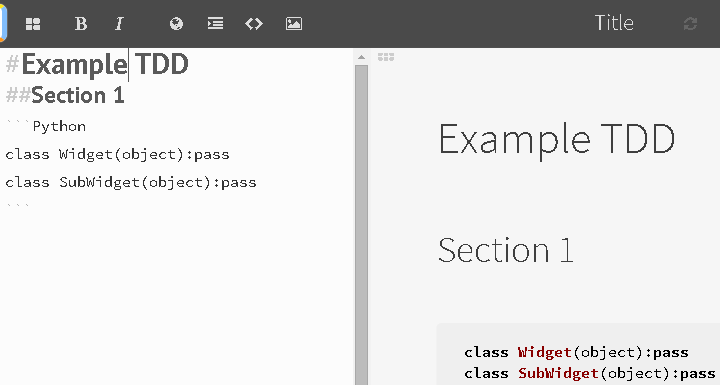
\includegraphics[scale=.5]{StackEdit.png}
		\caption{Editing Markdown Using StackEdit}
		\label{StackEdit}
	\end{figure}
	
	\subsubsection{Disadvantages}
	Markdown has drawbacks. It would need to be converted to HTML or a special program is needed for viewing nicely rendered documents.  There isn't the same support for markdown in text editors and IDEs as is available for HTML/CSS alone.  Also, there are multiple flavours of markdown, which could lead to compatibility problems unless a flavour, such as Github flavored markdown, were chosen as the standard within FINCAD.


\subsection{IPython Notebook - Qualifies}
	\subsubsection{Advantages}
	\subsubsection{Disadvantages}
	
	
	

\subsection{Latex - Eliminated}
	\subsubsection{Advantages}
	
	Many Quants are familiar with using Latex to format documents, and in particular mathematical equations.
	
	Latex's strength is in formatting mathematical equations and publishable documents.  However HTML and IPython can also format mathematical equations, and TDDs need only be easy to understand, not formatted to publish.
	
	\subsubsection{Disadvantages}
	A major disadvantage of Latex is that it would be totally unfamiliar to many programmers at FINCAD, and I would expect they would be unwilling to use Latex when HTML is familiar and likely to be much more useful in their future careers.
	
	For this reason, because I have not heard of TDDs ever being written using Latex, and because I am not that familiar with Latex myself, \emph{I exclude Latex from consideration in the remainder of this document}.




	

\section{Technical Details}
Let's first consider some simple examples of using these different languages/tools

\subsection{HTML}
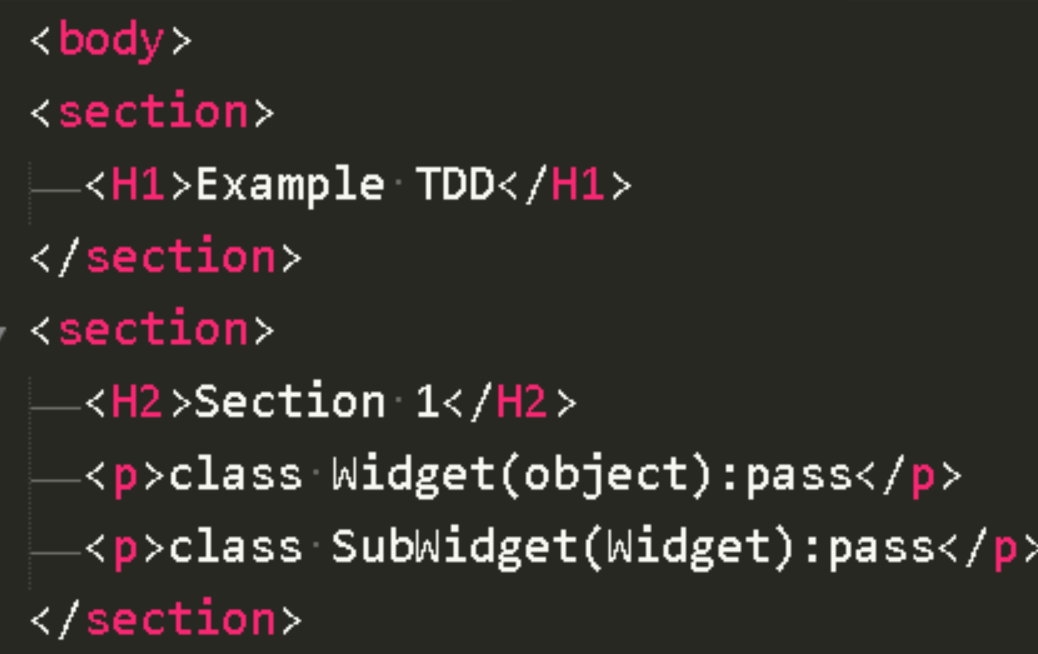
\includegraphics[scale=.25]{HTML_code.PNG}

As discussed, we have the following requirements and desiderata for creating TDDs:

\begin{enumerate}
	\item Requirements:
		\begin{enumerate}
			\item Amenable to code review
			\item Amenable to version control
		\end{enumerate}
	\item Desiderata:
		\begin{enumerate}
			\item Familiar
			\item Easy to use
			\item Easy to view
			\item Capable of expressing the ideas that we wish to convey
			
		\end{enumerate}
\end{enumerate}

\subsection{Comparison of HTML, Kompozer, Markdown, and IPython along these dimensions}

We now compare how HTML, Kompozer, Markdown, and IPython along each of these dimensions:

	\subsubsection{Amenable to code review and version control}
	
		
	
	\subsubsection{Familiar}
	
	\subsubsection{Easy to use}
	
	\subsubsection{Easy to view}
	
	\subsubsection{Capable of expressing the ideas that we wish to convey}



\end{document}
, however code reviews are usually only comprise a small part near the end of the design process, in which the design is officially signed off on.